\documentclass[a4paper]{article}
\usepackage[margin=1in]{geometry} 
% \usepackage{ctex}
\usepackage{tabularx}
\usepackage{lipsum}
\usepackage{enumerate}
\usepackage{amsfonts}
\usepackage{multirow}
\usepackage{graphicx}
\usepackage{siunitx}

\begin{document}
\begin{titlepage}
    \title{\textbf{Lab Report 3: Investigating how the length of string affects the period of circular motion}}
    \author{Eric Zhou}
    \date{\today}
    \maketitle
    %\tableofcontents
\end{titlepage}

\section{Introduction}

We have learned in physics that for an object of mass $m$ moving in a circular path of radius $r$, the required centripedal force (which is also the resultant force on the object) $F$ can be determined in the following formula:

$$F = m \omega^2 r = m {4\pi^2 \over T^2} r = m {v^2 \over r}$$

where $\omega$ is the angular speed, $T$ is the period, and $v$ is the velocity.

In this experiment, the main focus is the relationship between $T$ and $r$ when $m$ and $F$ are constant.

\textbf{Research question: What is the relationship between the radius of the path of circular motion and its period?}

\section{Background Knowledge}

People have not developed a systematic method to study the relationship between force and motion until the 17th century, when Newton's Laws of Motion were discovered and calculus is invented. Newton was the first person to come up with the formulae of force in circular motion. This study of the simplest form of non-linear motion enables people to investigate more about other more complecated non-linear motions, from celestrial bodies to microscopic particles.

The formulae of circular motion can actually be proved using Newton's Second Law and calculus.

\section{Hypothesis and Reasoning}

In this experiment, the second equation, $F = m {4\pi^2 \over T^2} r$ is the main focus. From that equation, we can easily find

$$FT^2 = m 4\pi^2 r$$

$$T^2 = {m 4\pi^2\over F} r$$

Therefore, we can hypothesize that:

\textbf{The period increases as the radius increases. The square of period should be directly proportional to the length of the string.}

\section{Experiment design}

\subsection{Variables}

\begin{itemize}
    \item Independent Variable: Length of the string $r$($10cm,20cm,30cm,40cm,50cm$. measured by a tape ruler)
    \item Dependent Variable: The time needed for the object to complete a whole circle.
    \item Controlled Variables: The mass, material of the object and the weight under the tube, the temperature and humidity of the environment, etc. They are listed in Table \ref{tab.ctrlvar}.
\end{itemize}

\begin{table}[ht!]
    \centering
    \caption[short]{Controlled Variables}
    \label{tab.ctrlvar}
    \begin{tabularx}{ \textwidth}{X X X X}
    \hline
    \hline
    Controlled Variable          & Spzecific Control Variable Value      & Reason to control                                                    & Method to control                                  \\
    \hline
    The mass and material of the weight &  Metal, approxmiately 50g     & Might affect centripedal force of the ball                           & Use the same object                                \\
    %\hline
    The mass and material of the ball   &  Plastic, approxmiately 5g    & Might affect centripedal force required to maintain the motion       & Use the same object                                \\
    %\hline
    Temperature                  & Local temperature. $31^oC\pm 1^oC$   & Might affect the air resistance.                                     & Complete the experiment during a short time period \\
    \hline
    \hline
    \end{tabularx}
\end{table}

\subsection{Materials}

\begin{itemize}
    \item 1 $\times$ plastic tube (the outershell of a pen)
    \item 1 $\times$ wool string with a plastic ball at the end (about $80$ cm long)
    \item 2 $\times$ weights (total mass $\approx 50g$)
    \item 1 $\times$ stopwatch
    \item 1 $\times$ photo capturing device
    \item 1 $\times$ meter rule
\end{itemize}

\subsection{Setup diagram}

The diagram of the experiment apparatus can be found in Figure \ref{fig.setup}. 

\begin{figure}[h]
    \centering
    \caption{Setup diagram}
    \label{fig.setup}
    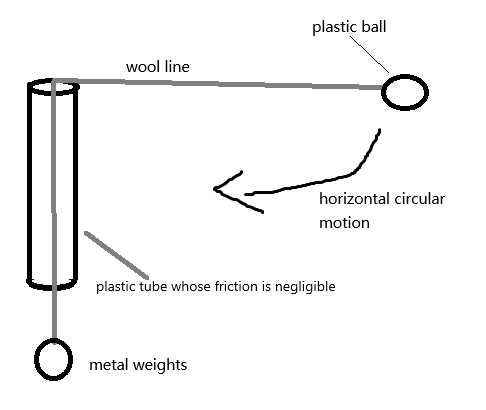
\includegraphics[width = 0.5\textwidth]{layout.png}
\end{figure}

\subsection{Method}

\begin{enumerate}[1.]
    \item Cross the string through the plastic tube. Make sure the plastic ball is at top.
    \item Attach the weights to the other end of the string.
    \item Adjust the position of the string to make its length above the tube is $r = 10cm$.
    \item Swing the tube until the plastic ball is doing constant circular motion. Make sure the string does not move relative to the tube during the process.
    \item Start the stopwatch.
    \item Count until the plastic ball has done 20 circular motions. Stop the stopwatch to find reading $t_1$.
    \item Repeat Step 6 twice to take down $t_2$ and $t_3$.
    \item Repeat Steps 2 $\sim$ 7 with $r = 20cm, 30cm, 40cm, 50cm$.
\end{enumerate}

\subsection{Risk Assessment}

This experiment is relatively safe with little potential hazard. It is still needed to avoid hitting others when swinging the ball.

\section{Results}
\subsection{Raw data}

We found the mass of the weights $M$ is $40.8\pm 0.5\SI{}{g}$, and the mass of the plastic ball $m$ is $5\pm 0.5\SI{}{g}$. Other data is listed in Table \ref{tab.raw}.

\begin{table}[ht!]\centering
    \caption{Raw data}
    \label{tab.raw}
    \begin{tabular}{lllll}
    \hline
    \multirow{2}{*}{Experiment} & \multirow{2}{*}{Length($r/\SI{}{cm}$)} & \multicolumn{3}{l}{Time for 20 oscillations($t/\SI{}{s}$)} \\
                                &                                        & \small Trial 1     & \small Trial 2    & \small Trial 3    \\ \hline
    1                           & $10 \pm 0.5$                           & $ 4.87 \pm 0.03$   & $ 4.44 \pm 0.03$  & $ 4.24 \pm 0.03$  \\
    2                           & $20 \pm 0.5$                           & $ 5.85 \pm 0.03$   & $ 5.72 \pm 0.03$  & $ 5.9 \pm 0.03$   \\
    3                           & $30 \pm 0.5$                           & $ 7.00 \pm 0.03$   & $ 7.19 \pm 0.03$  & $ 6.88 \pm 0.03$  \\
    4                           & $40 \pm 0.5$                           & $ 9.00 \pm 0.03$   & $ 9.10 \pm 0.03$  & $ 9.12 \pm 0.03$  \\
    5                           & $50 \pm 0.5$                           & $ 10.09 \pm 0.03$  & $ 10.16 \pm 0.03$ & $ 10.13 \pm 0.03$ \\ \hline
    \end{tabular}
\end{table}
% [0.07505553499465135, 0.05813776741499453, 0.049135381491199545, 0.043333333333333335, 0.03919647479510927]
\subsection{Processed data}

The predicted gradient is 

$${m4\pi^2 \over Mg} = 0.4926 (\pm 11\%)\SI{}{s^2/m} = 4.926\times 10^{-3} \pm 5.5\times 10^{-4}\SI{}{s^2/cm}$$

Other data is listed in Table \ref{tab.prod}.

\begin{table}[ht!]\centering
    \caption{Processed Data}
    \label{tab.prod}
    \begin{tabular}{llll}
        \hline
        Experiment & Avg. Time for 20 oscillations ($\bar{t}/\SI{}{s}$) & Period($T/\SI{}{s}$) & Period square ($T^2/\SI{}{s^2}$) \\ \hline
        1          & $ 4.52 \pm 6.97\% $                                & $ 0.23 \pm 6.97\% $  & $ 0.05 \pm 13.95\% $             \\
        2          & $ 5.82 \pm 1.55\% $                                & $ 0.29 \pm 1.55\% $  & $ 0.08 \pm 3.09\% $              \\
        3          & $ 7.02 \pm 2.21\% $                                & $ 0.35 \pm 2.21\% $  & $ 0.12 \pm 4.41\% $              \\
        4          & $ 9.07 \pm 0.66\% $                                & $ 0.45 \pm 0.66\% $  & $ 0.21 \pm 1.32\% $              \\
        5          & $ 10.13 \pm 0.35\% $                               & $ 0.51 \pm 0.35\% $  & $ 0.26 \pm 0.69\% $              \\ \hline
    \end{tabular}
\end{table}


\begin{figure}[h!]
    \centering
    \caption{$T^2 - r$ graph}
    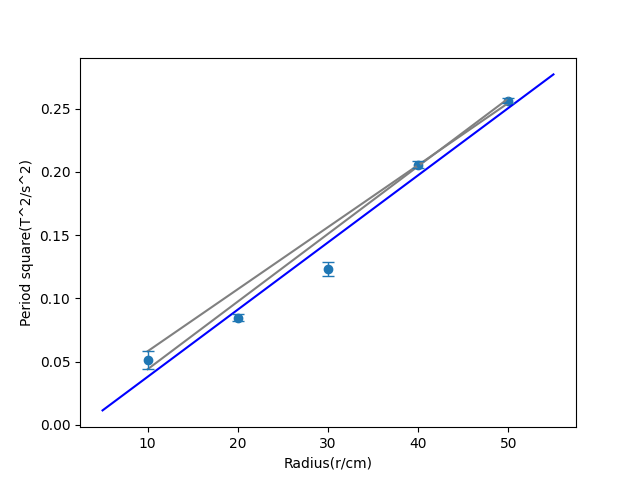
\includegraphics[width = 0.5\textwidth]{Figure_1.png}
\end{figure}

\subsection{Sample working}
To calculate the average time taken to completely pass through the photogate ($\bar{t}$):

$$\bar{t} = {{t_1+t_2+t_3}\over 3} = {{4.87+4.44+4.24} \over 3} s \approx 4.52 \SI{}{s}$$.
    
Percentage error of $\bar{t}$:
    
$$\%\Delta \bar{t} = {\Delta \bar{t} \over \bar{t}} \times 100\%= {\pm (4.87 - 4.24) \over 4.52} \times 100\% \approx 6.97\%$$

Since it is the time for $20$ oscillations, we divide the number by $20$ to get the period.

$$ T = {\bar{t} \over 20} \approx = 0.226\SI{}{s}$$

The percentage error remains unchanged. 

To plot $T^2$ against $r$. We have to square $T$ by $2$:

$$T^2 = (\SI{0.226}{s})^2 \approx 0.051 \SI{}{s^2}$$

Percentage error of $T^2$:

$$\%\Delta T^2 = 2{\%\Delta T} = 2\times 6.97\% = 13.94\%$$

\section{Discussion and conclusion}

The diagram shows a strong postive correlation of $T^2$ and $r$, and its best linear fit has

\begin{itemize}
    \item A slope of $0.005317$.
    \item A y-intercept of $-0.01527$.
\end{itemize}

As is mentioned in processed data section, the graph should have a gradient of approxmiately $4.926\times 10^{-3}$, and $5.317\times 10^{-3}$ is found There is an relative error of less than $7\%$, which is within the reasonable range of $11\%$ induced by the equipment. 

The y-intercept is expected to be zero, but $-0.01527$ is found. This might have resulted from the error of stopping the stopwatch.

Considering the small error, the results support our initial hypothesis. The period increases as the radius increases. The square of period should be directly proportional to the length of the string.

\section{Evaluation}

The experiment has been conducted successfully. However, there is still room for imporvement.

\begin{table}[!ht]
    \centering
    \caption{Evaluation }\label{tab:dummy-1}
    
      \begin{tabularx}{\textwidth} {XXX}
        \hline
        \hline
        \textbf{Limitation} & \textbf{Significancy} & \textbf{Improvement} \\
        \hline
        It's difficult to make sure the line is completely horizontal. & The $r$ measured may be longer than the actual ones. The force may be larger than the actual centripedal force.  & Take the factor into consideration. Find the angle to horizontal using a camera placed on a horizontal surface.\\
        %\hline
        The friction between the object and plastic tube may not be negligible. & The force applyed to the plastic ball is not completely from the weight, and may be inconsistant. & Lubricate the contact surface with appropriate substance or install a small trolly to reduce the friction. \\
        %\hline
        The center of the path is constantly moving when hand is used to exert force on the tube. & The motion is no longer circular motion by strict definition. & Use a machine to minimize the movement of the tube.\\
        The random error is too large. & May result in inacurracy. & Use better apparatus.\\
        \hline
        \hline
      \end{tabularx}
    
  \end{table}

\end{document}